The high level goal of \mEdhoc{} is to establish an authenticated security
context for the \mOscore{} security protocol.
%
The overall structure for reaching this goal is a three-message protocol in
the style of the \mNoise{} framework, outlined in
Figure~\ref{fig:edhocFramework}.
%
In the first message \mMsgone{}, the initiator provides the responder with an
ephemeral Diffie-Hellman half-key \mGx{} and dictates which authentication
methods should be used in the \mMethod{} element.
%
The responder may reject the choice of authentication methods.
%
In the second message \mMsgtwo{}, the responder provides its ephemeral
Diffie-Hellman half-key \mGy{} and authenticates itself to the initiator by
providing authentication information \mAuthr{}.
%
Finally, in the third message \mMsgthree{}, the initiator authenticates itself
to the responder by providing authentication information \mAuthi{}.
%
In addition to exchange of Diffie-Hellman half-keys and authentication data,
the messages also include agreement of parameters for the \mOscore{} security
context, such as encryption algorithm identifiers (\mSuites{}) and \mOscore{}
security context identifiers (\mCi{} and \mCr{}).
%
Optionally, messages may include application layer data \mAD{}, which enjoys
differing levels of protection depending on in which message it is sent.
%
As will be described below, when the authentication information is based on a
pre-shared key, the \mCredi{} and \mCredr{} credential identifiers are not
used.
%
Instead a single identifier for the pre-shared key is transmitted in message
\mMsgone{}.
%

\begin{figure}[!h]
%\begin{wrapfigure}{r}{20cm}
\centering
\scalebox{1}{
\tikzset{>=latex, every msg/.style={draw=thick}, every node/.style={fill=white,text=black}}
\begin{tikzpicture}
    \node (ini) at (0, 0) {Initiator};
    \draw [very thick] (0, -0.5) -- (0,-2.7);
    \draw [very thick] (7, -0.5) -- (7,-2.7);
    \node (res) at (7,0) {Responder};
    \msg{2em}{ini}{res}{\mMsgone: \mMethod, \mSuites, \mGx, \mCi, \mADone};
\msg{4em}{res}{ini}{\mMsgtwo: \mCi, \mGy, \mCr, [\mIdcredr, \mAuthr, \mADtwo]};
    \msg{6em}{ini}{res}{\mMsgthree: \mCr, [\mIdcredi, \mAuthi, \mADthree]};
    \draw [line width=2mm] (-0.75,-2.7) -- (0.75,-2.7);
    \draw [line width=2mm] (7-0.75,-2.7) -- (7+0.75,-2.7);
    \end{tikzpicture}}
\caption{Outline of the overall structure of \mEdhoc{}. Elements in square
brackets are encrypted and integrity protected.}
\label{fig:edhocFramework}
%\end{wrapfigure}
\end{figure}


A driving protocol design goal is to accommodate three credential types
a party may use to to authenticate itself to peers -- certificates, private keys
and static long-term Diffie-Hellman keys.
%
Depending on the credential types used by two peers running \mEdhoc{}, different
authentication methods are used.
%
The different authentication methods require different message content.
%
Specifically, the place holders \mAuthi{} and \mAuthr{} are constructed
differently depending on method.
%
So, it is natural to break down the description of \mEdhoc{} based on
these methods.
%

The authentication methods are digital signatures
(\mSig), challenge-response signatures based on static long-term Diffie-Hellman
keys (\mStat) and pre-shared symmetric keys (\mPsk).
%
We will sometimes refer to these authentication methods simply as methods.
%
Two parties may use different authentication methods in an \mEdhoc{} run.
%
Any combination of the \mSig{} and \mStat{} methods is possible, but when
\mPsk{} is used, both parties use \mPsk{}.
%
Overloading terminology, we refer to these combinations of authentication
methods also as methods, and
denote them \mSigSig, \mSigStat, \mStatStat, \mStatSig{} and \mPskPsk.
%
The first method in the name denotes the method used by the initiator of the
protocol run and the second denotes the method used by the responder.
%
Parties use mixed types of credentials in \mSigStat{} and \mStatSig{}, so
we call these methods mixed methods.
%
We refer to a method where at least one party uses \mSig{} as a \mSig-based
method and similarly for \mStat{} and \mPsk.
%

To put \mEdhoc{} in context we briefly discuss relations to
the protocols on which \mEdhoc{} is based before providing details on the
methods.
%

%-----------------------------------------------------------------------------
\subsection{Relations to \mSigma, \mOptls{} and \mNoise{}}
\label{sec:relationsToOtherProtocols}
The different methods use cryptographic cores from existing protocols to
establish the session key.
%
In conjunction with these cryptographic cores, \mEdhoc{} negotiates parameters
required for establishing a complete \mOscore{} security context.
%
Examples of such parameters are encryption algorithm identifiers discussed
previously.
%
We note that many key exchange protocols, e.g, \mSigma{}, has an explicit and
generic mechanism to securely negotiate such parameters, and that others can
easily be extended with such.
%
We also note that academic protocols, like \mSigma{} and \mOptls{} do not
specify exactly how messages and parameters are encoded, whereas an
industrially standardized protocol like \mEdhoc{} has to.
%
We leave those encoding details out when discussing the relations between
\mEdhoc{} and existing protocols.
%

%-----------------------------------------------------------------------------
\subsubsection{\mSigma{}}
\label{sec:sigma}
The \mSigSig{} method is closely modeled on \mSigma{}~\cite{sigma}.
%
Specifically, it is modeled on the \mSigmaI{} variant which provides identity
protection for the initiator.
%
However, \mSigSig{} deviates from \mSigmaI{} in some details, e.g.,
\mEdhoc{} uses Mac-then-Sign like \mTls{} instead of Sign-then-Mac.
%

Because \mSigSig{} is so close in spirit to \mSigmaI{} and is already carefully
analyzed by Bruni~et.~al.~\cite{DBLP:conf/secsr/BruniJPS18}, we will not focus
on it in this paper.
%
We do however model \mSigSig{} to the same extent and
verify its properties with the same care as the other methods.
%

%-----------------------------------------------------------------------------
\subsubsection{\mOptls{}}
\label{sec:optls}
The \mStat-based methods use challenge-response signatures using static
long-term Diffie-Hellman keys, and proceed along the lines of
\mOptls~\cite{cryptoeprint:2015:978}.
%
The challenge-response signature uses an ephemeral Diffie-Hellman half-key as
challenge, mixes this half-key with the static Diffie-Hellman key to generate
the session key and a symmetric temporary key to authenticate the session key
using an \mAead{}-transform~\cite{aead,rfc5116,DBLP:conf/eurosp/KrawczykW16}.
%
This authenticates one party to the other, which is sufficient for \mOptls in
that it only aims for server authentication.
%
In \mEdhoc, a party authenticating with with the \mStat{} method
essentially acts as an \mOptls{} client and the other party as an \mOptls{}
server.
%
\mEdhoc{} requires mutual authentication~\cite{ietf-lake-reqs-04} and achieves
this for \mStat{}-based methods by mirroring the actions just described, or
by using \mSig{}-based authentication for the other party.
%

The \mStatStat{} method can be thought of as interleaving two \mOptls{}
sessions, where the second \mEdhoc{} message carries both the response
message of the first \mOptls{} session and the request message of the second
\mOptls{} session.
%

Despite the close resemblances, there are differences.
%
For instance, \mEdhoc{} reuses the Diffie-Hellman half-key as a challenge to
save bandwidth, whereas \mOptls{} makes an explicit
point to use distinct elements for the Diffie-Hellman half-key and the
challenge, following the principle of separation of concerns.
%

\subsubsection{\mNoise{}}
The \mStatStat{} and \mPskPsk{} aim to follow the \mNoise{}
framework~\cite{perrin2016noise}.
%
This framework defines how to construct authenticated key exchange protocols,
known as patterns, using static long-term Diffie-Hellman keys or pre-shared
keys as
credentials.
%
Its goal is to harmonize among the many static long-term key Diffie-Hellman 
based key
exchange protocols, of which \mOptls{} is one.
%
\mNoise{} specifies how to derive keys, use transcript hashes to ensure
authentication of the message flow among other things.
%

The closest \mNoise{} pattern to the \mStatStat{} method appears to be the
XX pattern.
%

\knote{I don't believe the blue text is true. From the Noise spec it seems to
    me as if the message elements of XX and \mStatStat are exactly the same.
    XX does not describe any encrypted payload. "ee" means "create a DH-key from
    the two DH-half-keys" in \mNoise{}-language.
}
{\color{blue}
It can be seen that the first two messages of \mStatStat{}
correspond perfectly to the first two messages of the XX pattern of
the \mNoise{} framework.
%
However, in the third message, the XX pattern requires
the initiator to send their static key, followed by an encrypted payload using a
key derived from a combination of the static key and an ephemeral key.
%
In \mEdhoc{}, the static key and the payload are both encrypted in the same key, one depending on the key used for the second message, and on the static key of the initiator.
}

\mEdhoc{} does not use all functions of \mNoise{} exactly as prescribed though.
%
For example, \mNoise{} prescribes that the mixHash function, which corresponds
to the transcript hash of \mEdhoc{}, is called on pre-message public keys
during the initialization.
%
This would correspond to that \mEdhoc{} computes a first intermediate transcript
hash doing the same, which is not the case.
%
Because of this, one cannot automatically claim claim that \mEdhoc{} enjoys
the same properties as XX -- proofs may depend on functionality that \mEdhoc{}
does not have or performs differently.
%

%------------------------------------------------------------------------- sub
\subsection{Authentication methods}
\label{sec:methods}
We are now ready to dive into the details of the various methods supported by
\mEdhoc.
%
Although \mCose{} and \mCbor{} are important building blocks of \mEdhoc{}, and
we use their terminology in our \mTamarin{} model to better reflect the
\mSpec{}, our model does not cover
the details of encoding and \mCose{} interfaces.
%
For instance, on the abstraction level we work it suffices to consider
authenticated encryption with associated data (\mAead{})~\cite{aead} as a
function call.
%
Thus, we will not give more details on \mCose{} or \mCbor{}.
%

All methods make use of a common key hierarchy, which we will first describe.
%
We then move on to describe the methods and how they interact with the
key hierarchy.
%

%------------------------------------------------------------------------- sub
\subsubsection{Key hierarchy}
\label{sec:keyHierarchy}
Key derivations in \mEdhoc{} are done using the key derivation function
\mHkdf{}~\cite{rfc5869}.
%
The interface of \mHkdf{} provides two functions.
%
The first, \mHkdfExtract{}, is intended to construct a uniformly distributed
key material from random input and a seed.
%
The second, \mHkdfExpand{}, is used to generate keys from key material and a
seed.
%
Derived keys are then used as input to encryption and integrity protection
algorithms.
%
The seeds are used to bind the key material and keys to certain parameters.
%

The key hierarchy is rooted in an ephemeral Diffie-Hellman key \mGxy{}, i.e.,
the combination of the two half-keys \mGx{} and \mGy{}.
%
From that, it is successively constructed with each transmitted message.
%
Figure~\ref{fig:kdfdiagram} depicts a simplified version of the key hierarchy.
%
From \mGxy{} three intermediate keys are derived in a chain, one associated
with the second message,
\mPRKtwo{}, one associated with the third message, \mPRKthree{}, and a
final one from which the final session key material is derived, \mPRKfour{}.
%
The seed used for \mPRKtwo{} is dependent on which method is used.
%
For \mPskPsk{}, the pre-shared key is used as seed.
%
For all other methods the seed is empty.
%
In the \mPskPsk{} and \mSigSig{} methods, all three intermediate keys
are the same, i.e., $\mPRKtwo{} = \mPRKthree{} = \mPRKfour$.
%
For the three \mStat-based methods, however, they differ.
%
The differences comes from that when a party uses \mStat{}-based authentication,
the intermediate key \mPRKthree{} is dependent on the static long term key of
the party (possibly both) using \mStat{}-based authentication.
%

The result of an \mEdhoc{} run is not a key per se, but rather key material from
which actual encryption keys etc can be derived.
%


%The keys used for the \mAead{} encryptions are augmented with the suffix `e',
%for encrypting the ciphertext, or with the suffix `m', for generating the MAC
%(MACs only feature in the methods involving asymmetric keys). There are four
%keys -- \mKtwom, \mKtwoe, \mKthreem, and \mKthreeae. The suffixes in the names
%of the keys indicate which intermediate keys they are used to generate.
%\mPRKtwo{} is used to generate the key \mKtwoe{} along with the appropriate
%transaction hash. \mPRKthree{} is used for the keys \mKtwom{} and \mKthreeae,
%while \mPRKfour{} is used to generate \mKthreem.

\begin{figure}[htp]
\centering
% !TEX root =  edhocProtocol.tex
% Start the picture
\begin{tikzpicture}[%
    >=latex,              % Nice arrows; your taste may be different
    start chain=going below,    % General flow is top-to-bottom
    node distance=10mm and 60mm, % Global setup of box spacing
    every join/.style={norm},   % Default linetype for connecting boxes
    ]
% ------------------------------------------------- 
% A few box styles 
% <on chain> *and* <on grid> reduce the need for manual relative
% positioning of nodes
\tikzset{
terminput/.style={rounded corners, text width=6em},
term/.style={rounded corners},
  base/.style={draw, thick, on chain, on grid, align=center, minimum height=6ex},
  prk/.style={base, draw=Red3, fill=Red3!25, rectangle, text width=4em},
  %hkdfext/.style={base, draw=Green3, fill=Green3!25, isosceles triangle, isosceles triangle apex angle=60, anchor=base, shape border rotate=-90, text width=6em},
  hkdfext/.style={base, draw=Green3, fill=Green3!25, rectangle, text width=8em},
  %hkdfexp/.style={base, draw=orange, fill=orange!50, isosceles triangle, isosceles triangle apex angle=60, anchor=base, shape border rotate=-90, text width=6em},
  hkdfexp/.style={base, draw=orange, fill=orange!50, rectangle, text width=8em},
  keyb/.style={base, draw=Blue3, fill=Blue3!25, rectangle, text width=4em},
  % -------------------------------------------------
  norm/.style={->, draw, Blue3},
}
% -------------------------------------------------
% Start by placing the nodes
\node [prk] (p0) {$g^{xy}$};
\node [hkdfext, join] (h1) {\mHkdfExtract};
\node [prk, join] (p2) {\mPRKtwo};
\node [hkdfext, join] (h3) {\mHkdfExtract};
\node [prk, join] (p3) {\mPRKthree};
\node [hkdfext, join] (h5) {\mHkdfExtract};
\node [prk, join] (p4) {\mPRKfour};

\node [hkdfexp, shape border rotate=180, left= 3cm of p4] (h6) {\mHkdfExpand};
\node [keyb, join, left=3cm of h6] (k3) {\mKthreem};

\node [hkdfexp, shape border rotate=180, left= 3cm of p3] (h4) {\mHkdfExpand};
\node [keyb, join, left=3cm of h4] (k2) {\mKtwom};

\node [hkdfexp, shape border rotate=180, left= 3cm of p2] (h2) {\mHkdfExpand};
\node [keyb, join, left=3cm of h2] (k1) {\mKtwoe};

\node [hkdfexp, shape border rotate=180, below= 1cm of h4] (h8) {\mHkdfExpand};
\node [keyb, below=1cm of k2] (k2b) {\mKthreeae};
%\node [draw=none, fill=none, below=0.5cm of h4] (dummy) {};

\draw [->, norm] (p3.south) -- ++(0,-0.58) -- (h8);
\draw [->, norm] (h8) -- (k2b);
\draw [->, norm] (p2) -- (h2); 
\draw [->, norm] (p3) -- (h4); 
\draw [->, norm] (p4) -- (h6);
%\node [term, fill=Green3!25, below = -1.3cm of h1] (h1name) {\mHkdfExtract};
%\node [term, left = 1cm of h1name] (u1) {H1};
%\draw [->, dotted, shorten >=1mm] (u1) -- (h1name);
\node [terminput, right = 1cm of h1] (u1) {Initial salt};
\draw [->, dotted, shorten >=1mm] (u1) -- (h1);

%\node [term, fill=Green3!25, below = -1.3cm of h3] (h3name) {\mHkdfExtract};
%\node [term, left = 1cm of h3name] (u2) {H2};
%\draw [->, dotted, shorten >=1mm] (u2) -- (h3name);
\node [terminput, right = 1cm of h3] (u2) {Additional input};
\draw [->, dotted, shorten >=1mm] (u2) -- (h3);

\node [terminput, right = 1cm of h5] (u3) {Additional input};
\draw [->, dotted, shorten >=1mm] (u3) -- (h5);


%\node [term, fill=orange!50, below = -0.9cm of h2] (h2name) {\mHkdfExpand};
%\node [term, above = 1cm of h2name] (u3) {H3};
%\draw [->, dotted, shorten >=1mm] (u3) -- (h2);
\node [term, above = 1cm of h2] (u4) {\mTHtwo};
\draw [->, dotted, shorten >=1mm] (u4) -- (h2);

%\node [term, fill=orange!50, below = -0.9cm of h4] (h4name) {\mHkdfExpand};
%\node [term, above = 1cm of h4name] (u5) {H5};
%\draw [->, dotted, shorten >=1mm] (u5) -- (h4);
\node [term, above = 1cm of h4] (u5) {\mTHtwo};
\draw [->, dotted, shorten >=1mm] (u5) -- (h4);

\node [term, above = 0.7cm of h6] (u6) {\mTHthree};
\draw [->, dotted, shorten >=1mm] (u6) -- (h6);
\draw [->, dotted, shorten >=1mm] (u6) -- (h8);
%
% ------------------------------------------------- 
% 
%\path (h2.east) to node [near start, yshift=1em] {$n$} (c3); 
%  \draw [o->,lccong] (h2.east) -- (p8);
%\path (p3.east) to node [yshift=-1em] {$k \leq 0$} (c4r); 
%  \draw [o->,lcnorm] (p3.east) -- (p9);
% -------------------------------------------------
% 
%\path (h1.east) to node [near start, yshift=1em] {$n$} (c1); 
%  \draw [o->,lcfree] (h1.east) -- (c1) |- (p4);
%\path (h3.east) -| node [very near start, yshift=1em] {$n$} (c1); 
%  \draw [o->,lcfree] (h3.east) -| (c1);
%\path (p3.west) to node [yshift=-1em] {$k>0$} (c4); 
%  \draw [*->,lcnorm] (p3.west) -- (c4) |- (p3);
%\path (h4.east) -| node [very near start, yshift=1em] {$n$} (c6); 
%  \draw [o->,lcfree] (h4.east) -| (c6); 
%\path (h5.east) to node [near start, yshift=1em] {$n$} (c6); 
%  \draw [o->,lcfree] (h5.east) -| (c7); 
%\path (p4.east) to node [yshift=-1em] {$k \leq 0$} (c7); 
%  \draw [o->,lcfree] (p4.east) -- (c7)  |- (p9);
%\path (p4.west) to node [yshift=-1em] {$k>0$} (c5); 
%  \draw [*->,lcfree] (p4.west) -- (c5) |- (p5);
% -------------------------------------------------
% A last flourish which breaks all the rules
%\draw [->,MediumPurple4, dotted, thick, shorten >=1mm]
%  (p9.south) -- ++(5mm,-3mm)  -- ++(27mm,0) 
%  |- node [black, near end, yshift=0.75em, it]
%    {(When message + resources available)} (p0);
% -------------------------------------------------
\end{tikzpicture}
% =================================================

\caption{A diagram to illustrate the KDF key hierarchy}
\label{fig:kdfdiagram}
\end{figure}

With the key hierarchy outlined, we now describe each of the \mEdhoc{} methods.
%
As discussed above, the main differentiator between the methods is how
authentication is achieved.
%
We therefore focus on that.
%

\subsection{\mPskPsk{} method}
In this method, the initiator and responder are assumed to share a pre-shared
key (\mPsk) identified by \mIDPsk.
%
The message sequence is shown in Figure~\ref{fig:edhocpsk}.
%
The first message contains the \mIDPsk{} identifier.
%
The responder obtains the corresponding \mPsk{} and uses that to construct the
authentication data included in the second message.
%
The authentication data consists of the MAC in the \mAead{} transform used.
%
In the third message, the initiator uses the same technique to authenticate to
the responder.
%

Following custom, the transcript hash \mTH{} is tracking the data sent in the
messages.
%
Perhaps, one notable thing is that the transcript hash is lagging one message
behind.
%
That is, the transcript hash of the second message \mTHtwo{}, does not cover the
content of the second message.
%
The reason for this is that cannot cover the output of the \mAead{} transform,
because \mTHtwo{} is itself an input to it.
%
This is the same for all methods, but it turns out not to be an issue for the
properties we verify.
%
This is because the data not covered by the transcript hash is instead MACed or
signed.
%

\begin{figure}[!h]
\centering
\scalebox{.7}{
\tikzset{>=latex, every msg/.style={draw=thick}, every node/.style={fill=white,text=black}}
\begin{tikzpicture}
    \node (ini) at (0, 0) {Initiator};
    \draw [very thick] (0, -0.5) -- (0,-11);
    \draw [very thick] (11.5, -0.5) -- (11.5,-11);
    \node[below of=ini,fill=white,text=black] () {Knows $g,\ \mPsk,\ \mIDPsk,\ \mADone,\ \mADthree$};
    \node (res) at (11.5,0) {Responder};
    \node[below of=res] () {Knows $g,\ \mPsk,\ \mIDPsk,\ \mADtwo$};
    \action{4em}{ini}{Generates \mMethod,\ \mSuites,\ \mCi,\ $x$\\$\mGx = g^{x}$};
    \msg{8em}{ini}{res}{\mMsgone: \mMethod, \mSuites, \mGx, \mCi, \mIDPsk, \mADone};
    \action{9em}{res}{$
      \begin{array}{c}
        \text{Generates } \mCr,\ $y$\\
        \mGy = g^{y}\\
        \mTHtwo = \mHash(\mMsgone, g^{y})\\
        \mPRKtwo = \mHkdfExtract(\mPsk, g^{xy}) \\
        \mKtwoae = \mHkdfExpand(\mPRKtwo, \mTHtwo)
      \end{array}$};
    \msg{18em}{res}{ini}{\mMsgtwo: \mCi, \mGy, \mCr, $\overbrace{\mAead(\mKtwoae; \mTHtwo, \mADtwo)}^{\mCipher}$};
    \action{19em}{ini}{$
      \begin{array}{c}
       \mTHtwo = \mHash(\mMsgone, \mGy)\\
       \mPRKtwo = \mHkdfExtract(\mPsk, g^{xy}) \\
        \mKtwoae = \mHkdf(\mPRKtwo, \mTHtwo)\\
        \mTHthree = \mHash(\mTHtwo, \mCipher)\\
        \mPRKthree = \mPRKtwo \\
        \mKthreeae = \mHkdfExpand(\mPRKthree, \mTHthree)
      \end{array}$};
    
    \msg{28em}{ini}{res}{\mMsgthree: \mCr, \mAead(\mKthreeae; \mTHthree; \mADthree)};
    \action{29em}{res}{$
    \begin{array}{c}
    	\mPRKthree = \mPRKtwo \\
        \mKthreeae = \mHkdfExpand(\mPRKthree, \mTHthree)
    \end{array}$};
    \draw [line width=2mm] (-2,-11) -- (2,-11);
    \draw [line width=2mm] (9.5,-11) -- (13.5,-11);
    \end{tikzpicture}}
\caption{The \mPskPsk{} method of \mEdhoc. $\mAead(k; x; y)$ is used to denote
\mAead{} encryption where $k$ is the key, $x$ is associated data to be integrity
protected, and $y$ is the plaintext.}
\label{fig:edhocpsk}
\end{figure}

%------------------------------------------------------------------------- sub
\subsection{\mStat-based methods}
\mEdhoc{} provides three \mStat-based methods -- \mSigStat{}, \mStatStat{} and
\mStatSig{}.
%
The first message is common for all these methods, and only contains the
initiators ephemeral Diffie-Hellman half-key.
%
The content of the second and third messages depend on the method used.
%
In contrast to the \mPskPsk{} method, each party provide an identifier,
\mIdcredi{} and \mIdcredr{} respectively, for the credential they use (provided
that the peer cannot be assumed to know this from out of band information).
%
We now describe the specifics for each method.
%

%------------------------------------------------------------------------- sub
\subsubsection{\mSigStat}
The initiator uses the \mSig{} method, authenticating with a signature,
while the responder uses the \mStat{} method, authenticating with a
challenge-response signature.
%

In addition to being a Diffie-Hellman half-key, the value \mGx{} takes on the
function of challenge for the responder authentication.
%
To compute the response signature, the responder raises \mGx{} to the power of
its secret static long-term Diffie-Hellman key \mLtkr{}.
%
Assuming the discrete logarithm problem is hard in the underlying Diffie-Hellman
group, only the initiator and responder will be able to compute
$\mGx{}^\mLtkr{}$, and this value is woven in to the key hierarchy as depicted
in Figures~\ref{fig:kdfdiagram} and \ref{fig:edhocsigstat}.
%
The responder computes authentication data in the form of the \mAead{}
transform, similar to the \mPskPsk{} method, but the key is now dependent on
$\mGx{}^\mLtkr{}$.
%
Because the initiator can assume the only other party knowing
$\mGx{}^\mLtkr{}$ is the responder, the initiator can consider the responder
authenticated if the \mAead{} transform completes successfully.
%
The initator authenticates to the responder by a normal signature in the third
message.
%

\begin{figure}[!h]
\centering
%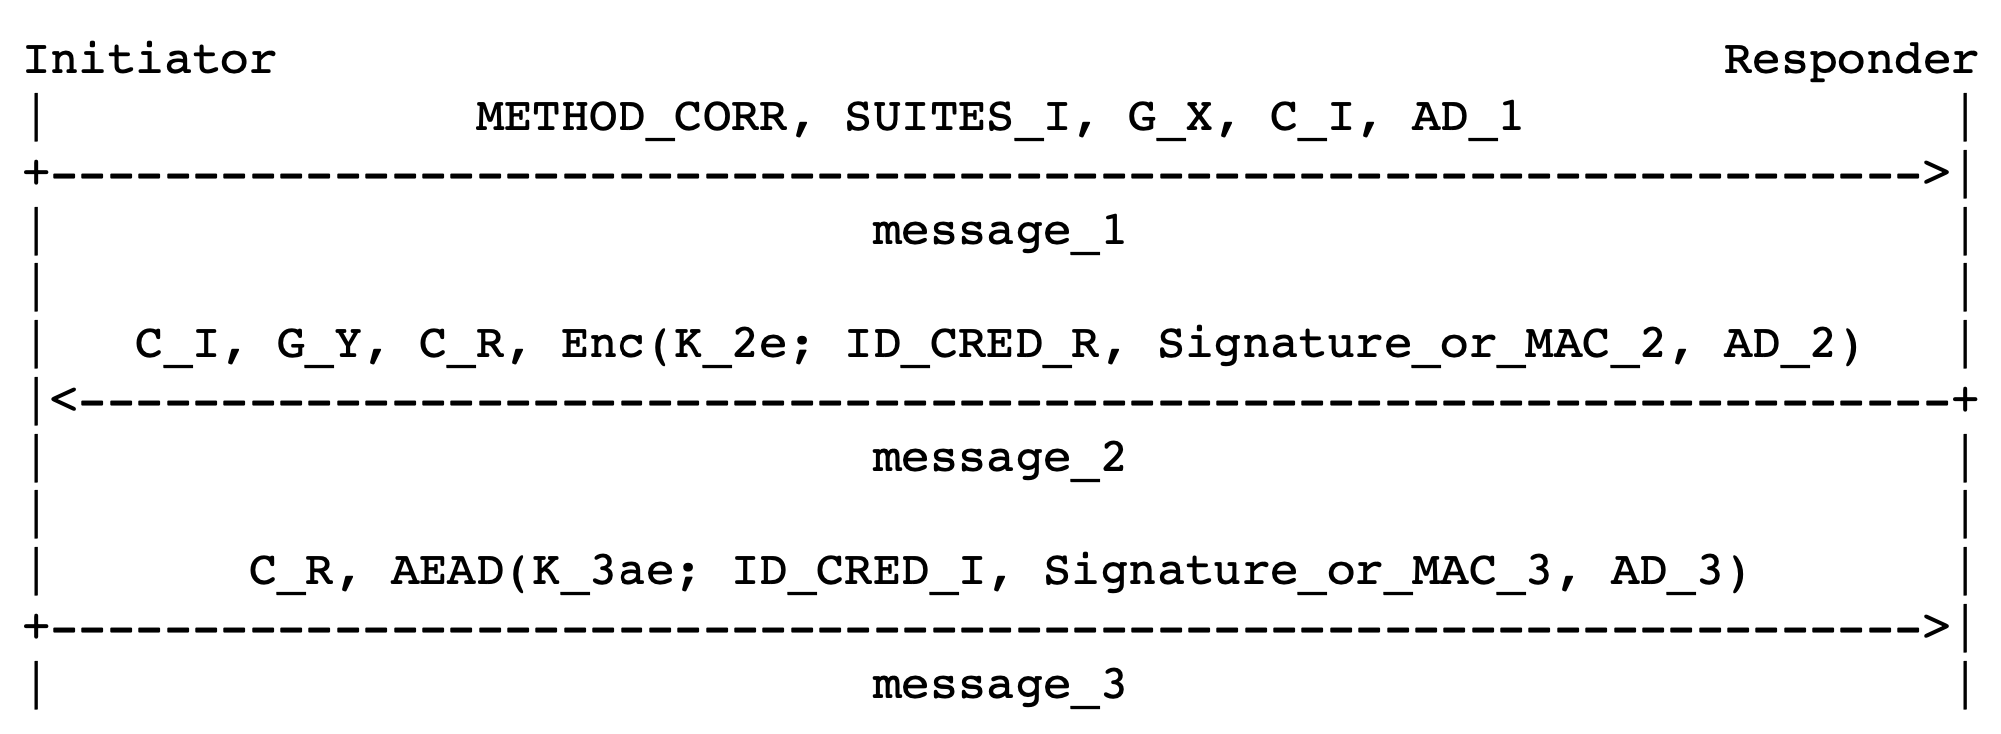
\includegraphics[scale=0.3]{Images/asym.png}
\scalebox{.7}{
\tikzset{>=latex, every msg/.style={draw=thick}, every node/.style={fill=white,text=black}}
\begin{tikzpicture}
    \node (ini) at (0, 0) {Initiator};
    \draw [very thick] (0, -0.5) -- (0,-15);
    \draw [very thick] (9, -0.5) -- (9,-15);
    \node[below of=ini,fill=white,text=black] {$
    \begin{array}{c}
    \text{Knows}\ $g$,\ \mCredi,\ \mLtki,\ \mIdcredi,\\
    \mIdcredr, \mADone,\ \mADthree
    \end{array}
    $};
    \node (res) at (9,0) {Responder};
    \node[below of=res] {$
    \begin{array}{c}
    \text{Knows}\ $g$,\ \mCredr,\ \mLtkr, \ \mIdcredr,\\
    \mIdcredi, \mADtwo
    \end{array}$};
    \action{5em}{ini}{Generates \mMethod,\ \mSuites,\ \mCi,\ $x$\\$\mGx = g^{x}$};
    \msg{10em}{ini}{res}{\mMsgone: \mMethod, \mSuites, \mGx, \mCi, \mADone};
    \action{11em}{res}{$
      \begin{array}{c}
        \text{Generates } \mCr,\ $y$\\
        \mGy = g^{y}\\
        \mTHtwo = \mHash(\mMsgone, \langle \mCi, \mGy, \mCr \rangle)\\
        \mPRKtwo = \mHkdfExtract(\textrm{``\phantom{}''}, g^{xy}) \\
        \mGrx = \mGx^{\mLtkr} \\
        \mPRKthree = \mHkdfExtract(\mPRKtwo, \mGrx) \\
        \mKtwom = \mHkdfExpand(\mPRKthree, \mTHtwo) \\
        \mMactwo = \mAead(\mKtwom; \langle \mIdcredr, \mTHtwo, \mCredr, \mADtwo \rangle; \textrm{``\phantom{}''}) \\
        \mKtwoe = \mHkdfExpand(\mPRKtwo, \mTHtwo)
      \end{array}$};
    \msg{26em}{res}{ini}{\mMsgtwo: \mCi, \mGy, \mCr, $\overbrace{\mKtwoe\ \mXor\ \langle \mIdcredr, \mMactwo, \mADtwo \rangle}^{\mCipher}$};
    \action{27em}{ini}{$
      \begin{array}{c}
        %\mTHtwo = \mHash(\mMsgone, \langle \mCi, \mGy, \mCr \rangle) \
        \mPRKtwo = \mHkdfExtract(\textrm{``\phantom{}''}, g^{xy}) \\
        %\mKtwoe = \mHkdfExpand(\mPRKtwo,\mTHtwo)\\
        \mGrx = \mCredr^{x} \\
        \mPRKfour = \mPRKthree = \mHkdfExtract(\mPRKtwo, \mGrx) \\
        %\mKtwom = \mHkdfExpand(\mPRKthree, \mTHtwo) \\
        \mKthreeae = \mHkdfExpand(\mPRKthree, \mTHtwo) \\
        \mTHthree = \mHash(\mTHtwo, \mCipher, \mCr)\\
        \mKthreem = \mHkdfExpand(\mPRKfour, \mTHthree) \\
        \mMacthree = \mAead(\mKthreem; \langle \mIdcredi, \mTHthree, \mCredi, \mADthree \rangle; \textrm{``\phantom{}''}) \\
        \mSigthree = \mSign(\mLtki; \langle \mIdcredi, \mTHthree, \mCredi, \mADthree \rangle, \mMacthree \rangle)
      \end{array}$};
    \msg{39em}{ini}{res}{$\mMsgthree: \mCr, \mAead(\mKthreeae; \mTHthree; \langle \mIdcredi, \mSigthree, \mADthree \rangle$)};
    \action{40em}{res}{$
    \begin{array}{c}
        \mTHthree = \mHash(\mTHtwo, \mCipher, \mCr)\\
        \mKthreem = \mHkdfExpand(\mPRKthree, \mTHthree) \\
        \mKthreeae = \mHkdfExpand(\mPRKthree, \mTHthree)
    \end{array}$};
    \draw [line width=2mm] (-2,-15) -- (2,-15);
    \draw [line width=2mm] (7,-15) -- (11,-15);
    \end{tikzpicture}}
    \caption{The \mSigStat{} method of \mEdhoc. \mCredi{} and \mLtki, and
        \mCredr{} and \mLtkr{} are two public-private key pairs. \mCredi{} and
    \mLtki{} must be signature keys in the \mSig{} method. $\mSign(k; x)$ is
    used to denote the signing of message $x$ using key $k$.}
\label{fig:edhocsigstat}
\end{figure}

\subsubsection{\mStatStat}
In this method, both the initiator and the responder use the \mStat{}
authentication method.
%
The responder executes the same as in the previous subsection, except for how
authenticating the initiator.
%
Because the initiator usess the \mStat{} method, it authenticates using a
challenge-response signature, using \mGy{} as the challenge and raising that to
the power of the initiator's secret static long-term Diffie-Hellman key
\mLtki{}.
%
The result $\mGy{}^\mLtki{}$ is woven into the key hierarchy in the same way as
$\mGx{}^\mLtkr{}$.
%
In contrast to the \mSigStat{} method, both parties' secret static long-term
Diffie-Hellman keys here affect the key hierarchy, and ultimately the session
key material.
%
The initiator computes authentication data using the \mAead transform
and includes that in the third message for the responder to verify.
%
As expected the initiator's behavior mirrors the \mStat{} authentication method
used by the responder in the previous subsection.

%------------------------------------------------------------------------- sub
\subsubsection{\mStatSig}
Here, the responder runs the \mSig{} method, while the initiator runs the \mStat{} method. Thus, the second message, sent by the responder to the initiator needs an extra layer of signing. 

The intermediate keys are now generated in a slightly different manner, since
the responder is running \mSig. \mPRKtwo{} is still generated by running the KDF
on the empty salt and \mGxy. However, \mPRKthree{} is now equal to \mPRKtwo.
\mKtwom{} and \mKtwoe{} follow the same guidelines as earlier, but with these
values of \mPRKtwo{} and \mPRKthree. The responder constructs \mMactwo{} as earlier.

Once \mMactwo{} has been constructed, the responder runs the signature algorithm
with a \mCose{} object. This object has \mIdcredr{} as protected data, a
concatenation of \mTHtwo, \mCredr, and \mADtwo{} as external data, and the payload \mMactwo. This is signed using the responder's private authentication key to obtain \mSigtwo.

The outer encryption object is constructed by considering a plaintext consisting
of \mCredr, \mSigtwo{} (instead of \mMactwo), and \mADtwo. The key \mKtwoae{} is \mXor-ed with this plaintext to get a ciphertext, and the responder sends \mGy, \mCr, and this ciphertext to the initiator as the second message.

The initiator generates the intermediate key \mPRKtwo by running the KDF on
empty salt and \mGxy{} and sets \mPRKthree{} equal to \mPRKtwo. These are used
for generating the \mKtwom{} and \mKtwoe{} for decrypting the message received
from the responder. The intermediate key \mPRKfour{} is generated by giving as
input to \mHkdfExtract{} \mPRKthree{} as salt, and \mGiy{} as IKM -- \mGiy{} is
obtained as in the \mStatStat{} method.

Now, to generate the encryption keys, the initiator generates \mKthreem{} by
passing \mPRKfour{} and \mTHthree{} to the KDF. \mKthreeae{} is generated by
running the KDF on \mPRKthree{} and \mTHthree. There is no signature, and the
message is constructed exactly as in the \mStatStat{} case, except with these
values of \mKthreem{} and \mKthreeae.

In order to decrypt the message received from the initiator, the responder needs
to generate keys. \mKthreeae{} is straightforward, but in order to generate
\mKthreem, the responder needs \mPRKfour. To generate this intermediate key, the
responder runs \mHkdfExtract{} on \mPRKthree{} as salt, and uses as IKM \mGiy,
which is obtained by exponentiating the initiator's public authentication key to
the responder's ephemeral secret \mGy. As earlier, this is an asymmetric key
used for ``decrypting'' the \mGiy{} used by the initiator to construct its \mPRKfour. This method is illustrated in Figure~\ref{fig:edhocstatsig}.

\begin{figure}[!h]
\centering
%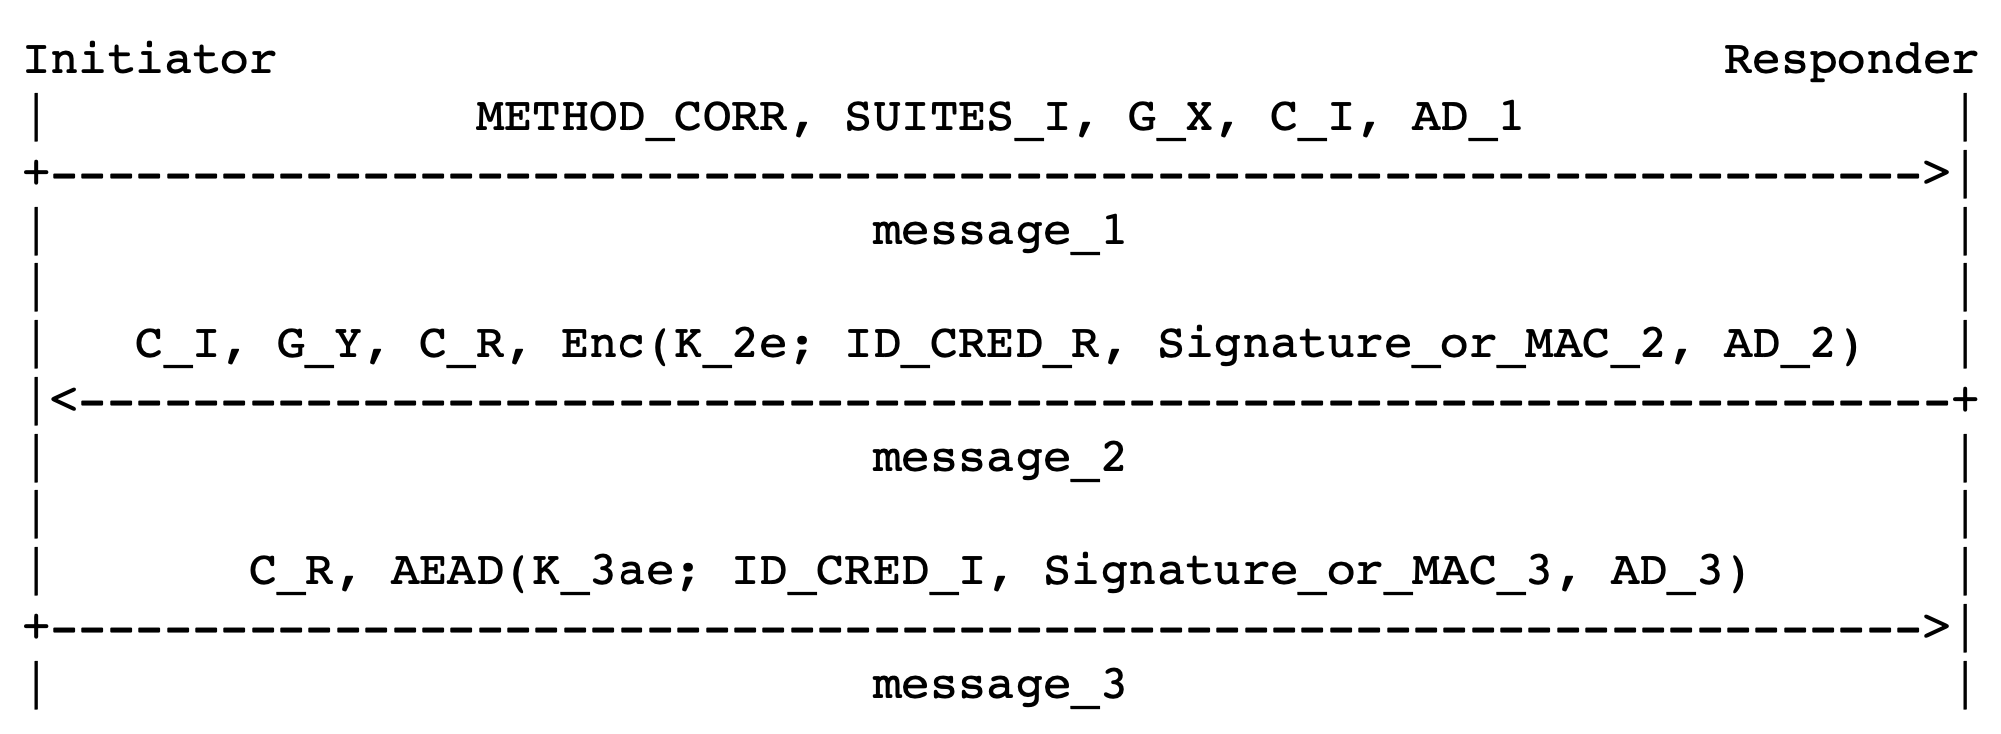
\includegraphics[scale=0.3]{Images/asym.png}
\scalebox{.7}{
\tikzset{>=latex, every msg/.style={draw=thick}, every node/.style={fill=white,text=black}}
\begin{tikzpicture}
    \node (ini) at (0, 0) {Initiator};
    \draw [very thick] (0, -0.5) -- (0,-15.2);
    \draw [very thick] (9, -0.5) -- (9,-15.2);
    \node[below of=ini,fill=white,text=black] {$
    \begin{array}{c}
    \text{Knows}\ $g$,\ \mCredi,\ \mLtki,\ \mIdcredi,\\
    \mIdcredr, \mADone,\ \mADthree
    \end{array}
    $};
    \node (res) at (9,0) {Responder};
    \node[below of=res] {$
    \begin{array}{c}
    \text{Knows}\ $g$,\ \mCredr,\ \mLtkr,\ \mIdcredr,\\
    \mIdcredi, \mADtwo
    \end{array}$};
    \action{5em}{ini}{Generates \mMethod,\ \mSuites,\ \mCi,\ $x$\\$\mGx = g^{x}$};
    \msg{10em}{ini}{res}{\mMsgone: \mMethod, \mSuites, \mGx, \mCi, \mADone};
    \action{11em}{res}{$
      \begin{array}{c}
        \text{Generates } \mCr,\ $y$\\
        \mGy = g^{y}\\
        \mTHtwo = \mHash(\mMsgone, \langle \mCi, \mGy, \mCr \rangle)\\
        \mPRKthree = \mPRKtwo = \mHkdfExtract(\textrm{``\phantom{}''}, g^{xy}) \\
        \mKtwom = \mHkdfExpand(\mPRKthree, \mTHtwo) \\
        \mMactwo = \mAead(\mKtwom; \langle \mIdcredr, \mTHtwo, \mCredr, \mADtwo \rangle; \textrm{``\phantom{}''}) \\
        \mSigtwo = \mSign(\mLtkr; \langle \langle \mIdcredr, \mTHtwo, \mCredr, \mADtwo \rangle, \mMactwo \rangle)\\
        \mKtwoe = \mHkdfExpand(\mPRKtwo, \mTHtwo)
      \end{array}$};
    \msg{25em}{res}{ini}{\mMsgtwo: \mCi, \mGy, \mCr, $\overbrace{\mKtwoe\ \mXor\ \langle \mIdcredr, \mSigtwo, \mADtwo \rangle}^{\mCipher}$};
    \action{26em}{ini}{$
      \begin{array}{c}
        \mPRKthree = \mPRKtwo = \mHkdfExtract(\textrm{``\phantom{}''}, g^{xy}) \\
        \mGiy = \mGy^{\mLtki} \\
        \mPRKfour = \mHkdfExtract(\mPRKthree, \mGiy) \\
        \mTHthree = \mHash(\mTHtwo, \mCipher, \mCr)\\
        \mKthreem = \mHkdfExpand(\mPRKfour, \mTHthree) \\
        \mMacthree = \mAead(\mKthreem; \langle \mIdcredi, \mTHthree, \mCredi, \mADthree \rangle; \textrm{``\phantom{}''}) \\
        \mKthreeae = \mHkdfExpand(\mPRKthree, \mTHthree) \\
      \end{array}$};
    \msg{37em}{ini}{res}{$\mMsgthree: \mCr, \mAead(\mKthreeae; \mTHthree; \langle \mIdcredi, \mMacthree, \mADthree \rangle$)};
    \action{38em}{res}{$
    \begin{array}{c}
       \mGiy = \mCredi^{y} \\
       \mPRKfour = \mHkdfExtract(\mPRKthree, \mGiy) \\
       \mTHthree = \mHash(\mTHtwo, \mCipher, \mCr)\\
        \mKthreem = \mHkdfExpand(\mPRKfour, \mTHthree) \\
        \mKthreeae = \mHkdfExpand(\mPRKthree, \mTHthree)
    \end{array}$};
    \draw [line width=2mm] (-2,-15.2) -- (2,-15.2);
    \draw [line width=2mm] (7,-15.2) -- (11,-15.2);
    \end{tikzpicture}}
\caption{The \mStatSig{} method of \mEdhoc}
\label{fig:edhocstatsig}
\end{figure}

\subsection{\mSigSig{} method}
In this method, both parties run the \mSig{} method, and therefore, both the
second and third messages need to be signed before being encrypted via \mAead.
The intermediate key \mPRKtwo{} is generated as usual, by sending the empty salt
and the shared secret to the KDF, and both \mPRKthree{} and \mPRKfour{} are set equal to \mPRKtwo. The second message looks like the one from the \mSigStat{} method described above, while the third looks like the one from the \mStatSig{} method.

%\subsection{Negotiating a cipher suite and method and correlation parameters}
%\label{sec:ciphersuite}
%Recall that we mentioned that the first message contains a list of cipher suites, ranked according to the preference of the initiator. What does a cipher suite actually contain? An \mEdhoc{} cipher suite consists of an ordered set of \mCose{} algorithms: an \mAead{} algorithm, a hash algorithm, an ECDH curve, a signature algorithm, a signature algorithm curve, an application \mAead{} algorithm, and an application hash algorithm from the \mCose{} Algorithms and Elliptic Curves registries.  
%
%There are four supported cipher suites in \mEdhoc{} -- we refer the reader to Section 3.4 of~\cite{selander-lake-edhoc-01} for the specifics of the algorithms allowed therein. Each cipher suite is identified by one of four predefined integer labels (0--3). Some algorithms are not used in some methods.  The signature algorithm and the signature algorithm curve are not used in methods without signature authentication (i.e. in \mPskPsk{} and \mStatStat).
%
%In order to keep the presentation clean, we have omitted the cipher suite negotiation process from the description of the methods. However, this process happens as follows, at the beginning of every method, once the responder receives the first message. The initiator proposes an ordered list of cipher suites they support. This list presented in descending order to the responder who either accepts the topmost entry in this list (if they also support that suite) or makes a counter-proposal, namely the topmost entry which they support from the remaining part of the list. If there is no such entry the responder can reject, and the protocol does not continue. Similarly, the responder can reject the initiator's choices for the method and correlation parameters as well -- in the case of a reject for either of these values, the protocol aborts.


\subsection{Deriving an OSCORE context}
\mEdhoc{} is often used to set up parameters for \mOscore. In this case, the
parties make sure that the connection identifiers are distinct, i.e. $\mCredi
\neq \mCredr$, since these are used as \mOscore{} sender IDs. If the initiator
plays the role of the CoAP client, and the responder the role of the CoAP
server, the client gets the sender ID \mCredr{} and the server the ID \mCredi{} (the identifiers are swapped). The \mAead{} and hash algorithms for \mOscore{} stay the same as those used for the selected cipher suite in \mEdhoc, while the master secret for \mOscore{} is derived using the key length of the \mAead{} algorithm of \mEdhoc. 

\subsection{Expected security properties}
In this section, we list all the claims made by the authors of~\cite{selander-lake-edhoc-01} regarding the security properties satisfied by \mEdhoc. We will revisit these claims when we discuss the formal modeling and verification of \mEdhoc{} in Section~\ref{sec:formalization}. 

The following are the claims made by the authors of~\cite{selander-lake-edhoc-01}. 

\mEdhoc{} inherits some security properties from the \mSigma{} protocol. These are perfect forward secrecy, mutual authentication with aliveness, consistency, peer awareness (to the responder, but not to the initiator), identity protection, and Key Compromise Impersonation (KCI) resistance.

All methods other than \mPskPsk{} offer identity protection of the initiator against active attacks and that of the responder against passive attacks. The roles should be assigned to protect the more sensitive identity. This is usually the entity whose identity cannot be inferred from information in the lower layers.

\mEdhoc{} also provides protection against replay attacks by the attacker. The attacker also cannot affect any negotiated parameters. A single session of \mEdhoc{} enables the responder to verify that the selected cipher suite is the most preferred of the initiator which is supported by both parties, even though there is no negotiation of cipher suites per se.

In order to reduce the chances of pervasive monitoring, \mEdhoc{} only supports methods with perfect forward secrecy. One way to limit the effect of breaches is to minimize the use of symmetrical group keys for bootstrapping. \mEdhoc, therefore, uses raw public keys and self-signed certificates instead of symmetrical group keys for bootstrapping.

For the \mPskPsk{} method, compromising \mPsk{} lets the attacker impersonate either party in \mEdhoc{} exchanges with the other. For the other methods, compromising the private authentication keys of one party lets the attacker impersonate only the compromised party in exchanges with other parties. In particular, it does not let the attacker masquerade as any other parties in communications with the compromised party. 

Compromise of the \mHkdf{} input parameters (\mGxy{} shared secret and/or \mPsk) leads to all session keys derived from that shared secret being deemed compromised. However, the compromise of one session key does not affect other session keys. If the long-term keys (\mPsk{} or private authentication keys) are compromised, this does not affect the security of instances of \mEdhoc{} which have completed prior to compromise. 

In this paper, we verify secrecy, authentication, session independence, perfect forward secrecy, key-compromise impersonation, and some flavor of post-compromise security. We will also discuss, in Section~\ref{sec:discussion} what it means for these properties to hold about this model.
